\subsection{Classes}
			
\subsubsection{Action}
This is an action that can be executed in a task of the workflow.
			
\begin{figure}[htbp]
\centering
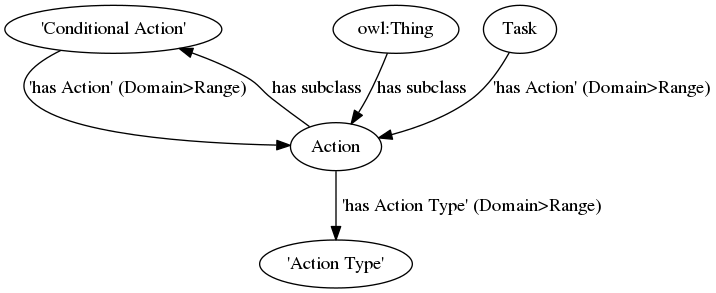
\includegraphics[width=\textwidth]{figures/action.png}
\caption{FIXME!}
\label{action}
\end{figure}

\subsubsection{Action Type}
This resource defines the type of the action that will be executed. It
distinguishes between types of actions such as shell functions, user input,
waiting, etc.
			
\begin{figure}[htbp]
\centering
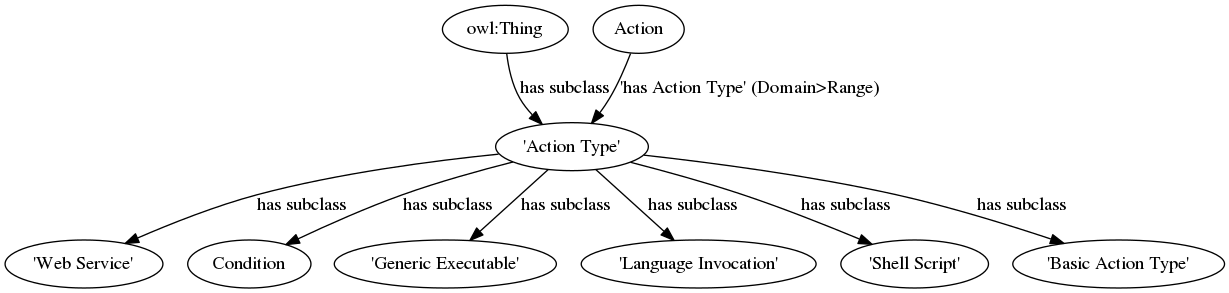
\includegraphics[width=\textwidth]{figures/actionType.png}
\caption{FIXME!}
\label{actionType}
\end{figure}
			
			\subsubsection{
			Basic Action Type
			}
			The Basic Action Type is the base class for basic actions that are typically considered native actions of workflow engines that execute workflows. This includes actions such as moving files or doing simple reductions.
			\subsubsection{
			Boolean Condition
			}
			Boolean Conditions evaluate boolean statements, such as "if" statements.
			\subsubsection{
			Common Workflow Language Tool
			}
			This node represents a Common Workflow Language (CWL) Tool, which is a description of a command line tool used in CWL workflows.
			\subsubsection{
			Condition
			}
			Conditional Actions Types indicate that the action described by this type executes for the purpose of evaluating some logical condition, such as a boolean statement, a loop, a cycle, or waiting (polling, checking) for feedback from an external agent.
			\subsubsection{
			Conditional Action
			}
			Conditional Actions are actions that execute conditionally for either conditional tasks (i.e. - as part of the workflow) or as alternative execution flows when the task enters a different state.

Conditional actions assigned to tasks indicate that the primary action of the task should be executed according to the conditional action type until the condition action evaluates to true.
			\subsubsection{
			Cycle
			}
			A Cycle describes an action that exits when a condition describing the end of a cycle has been met. Where a loop action type describes execution over a range, a cyclic action type checks for the completion of a task cycle.
			\subsubsection{
			Generic Executable
			}
			The Executable Action Type is the base class for actions that require executing generic programs on the system.
			\subsubsection{
			External Agent Condition
			}
			The External Agent Condition describes an action that waits conditionally on feedback from an external agent, including a human or an external service. Tasks can block themselves to wait on feedback, but in some cases an explicit task may exist for a user can that can be described and explicitly executed in the workflow.
			\subsubsection{
			Fortran Function
			}
			The Fortran Function Action Type is the base class for actions that require executing a function in the Fortran programming language.
			\subsubsection{
			Java Class
			}
			The Java Class Action Type is the base class for actions that require executing a class in the Java programming language. Action Targets for this type should point to a single method in the class that will create all necessary state and configure the system before executing. Thus, to execute a class Car, it may make sense to call a builder class such as "CarBuilder.runCar" instead.
			\subsubsection{
			Language Invocation
			}
			This action type represents actions to invocation language-specific calls or executions as part of the workflow. This could include, for example, executing a method on a native Java class, or a Fortran function or subroutine, or an R function.
			\subsubsection{
			Loop
			}
			The Loop describes an action that exits when a condition describing the end of a loop has been met. The loop executes over a range, and differs from a cyclic action type because the latter checks for the completion of a task cycle.
			\subsubsection{
			Parallel Loop
			}
			A Parallel Loop Condition indicates that the loop may be executed in parallel (i.e. - that the iterations of the loop are independent).
			\subsubsection{
			Python Script
			}
			The Python Script Action Type is the base class for actions that require executing a script in the Python programming language.
			\subsubsection{
			RESTful Web Service
			}
			This action types describes Representational State Transfer (RESTful) web services.
			\subsubsection{
			SOAP Web Service
			}
			This action types describes Simple Object Access Protocol (SOAP) web services.
			\subsubsection{
			Shell Script
			}
			The Shell Script action type is for actions that require executing shell scripts on systems that support shells.
			\subsubsection{
			State Change
			}
			A State Change is executed under the condition that a task experiences a state change.
\subsubsection{Task}

Tasks are executed by workflows. They are modeled as the combination of an
action and properties defining the way that action should be executed.

Tasks may also be assigned conditional actions that evaluate when a certain
condition has been met based on the execution of the primary action with its properties.

\begin{figure}[htbp]
\centering
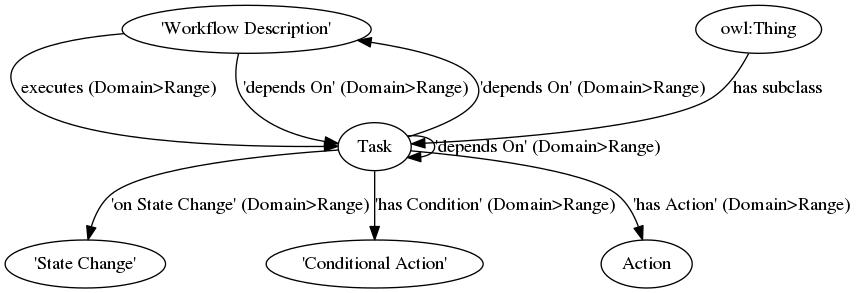
\includegraphics[width=\textwidth]{figures/task.png}
\caption{FIXME!}
\label{task}
\end{figure}


			\subsubsection{
			WSDL Web Service
			}
			This action types describes Web Service Description Language (WSDL) web services.
			\subsubsection{
			Web Service
			}
			The Web Service Action Type is the base class for actions that require executing remote web services.
\subsubsection{Workflow Description}

This class provides a description of the data and tasks that make up a
workflow. It describes a collections of tasks that are executed to accomplish
an activity with certain goals according to various properties and possibly
using some data.

\begin{figure}[htbp]
\centering
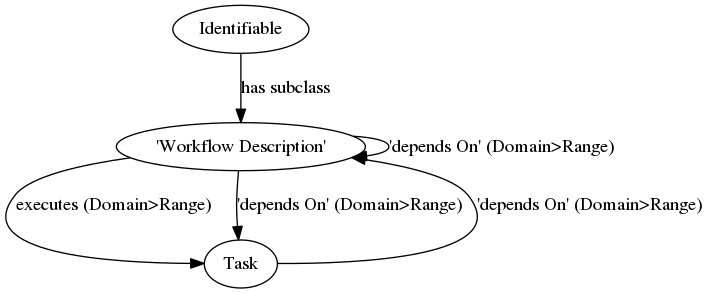
\includegraphics[width=\textwidth]{figures/workflowDescription.png}
\caption{FIXME!}
\label{workflow-description}
\end{figure}


\subsection{Object Properties}
			\subsubsection{
			depends On
			}
			This property indicates that the task (domain) depends on the successful execution of the range, which is another task or set of tasks.

It is possible to declare multiple instances of this object property such that one task will depend on the successful execution of multiple tasks.
			\subsubsection{
			executes
			}
			This property links a workflow description to a task that it should execute.
			\subsubsection{
			has Action
			}
			This object property denotes that the task (domain) uses the action (range) to which it points.
			\subsubsection{
			has Action Target
			}
			This tag describes the target (program, function, web service, etc.) that the action should execute. Its domain is tied to Action, but its range is open to accommodate what ever the type of the target is.
			\subsubsection{
			has Action Type
			}
			This property links a concrete action type to the subject, which must be an action instance.
			\subsubsection{
			has Condition
			}
			This property indicates that the conditional task (domain) is subject to the completion only if the conditional action (range) executes successfully.
			\subsubsection{
			has Properties
			}
			This property indicates that the task (domain) has the properties described by the range. The range is open because the type of the properties may be undefined.
			\subsubsection{
			on State Change
			}
			This property links a task (domain) to a state change action (range) that it should execute when its state changes.
\subsection{Datatype Properties}
			\subsubsection{
			has Host
			}
			This property describes the host on which a task or workflow should be executed.
			\subsubsection{
			has State
			}
			This data property describes the present state of the task or workflow.
			\begin{itemize}
			  \item \textbf{Initialized} - This pseudostate indicates that the state
			  machine has fully initialized. In practice, full and successful
			  initialization results in an immediate local transition to Ready.
			  \item \textbf{Failed} - This state indicates that an unexpected failure
			  happened while executing the task.
			  \item \textbf{Reviewing} - The Reviewing state is entered when a task
			  needs to spend a large amount of time to review information received for
			  pre-, post-, or in-situ processing that is required to execute the task.
			  Once the review is complete, the task will transition into the Executing
			  state in the ideal primary flow.
			  \item \textbf{Waiting} - Tasks in the waiting state are waiting on
			  resources to be properly allocated, including either compute or data
			  resources.
			  \item \textbf{WaitingForInfo} - Tasks in the WaitingForInfo state are
			  waiting on information from an external agent.
			  \item \textbf{Finished} - This is the terminal state for the task and
			  indicates that it has been completely executed.
			  \item \textbf{Executing} - This state indicates that the task is presently
			  executing the work assigned to it.
			  \item \textbf{Ready} - The ready state indicates that the task can be
			  executed and that all initialization has completed, or that execution has
			  finished and the task is ready to be executed again.
			\end{itemize}